\chapter{Geometrie auf der Kugeloberfläche\label{chapter:kugel}}
\lhead{Geometrie auf der Kugeloberfläche}
\begin{refsection}
\chapterauthor{Melina Staub und Fabian Schmid}


\section{Einleitung}

\begin{figure}
\centering
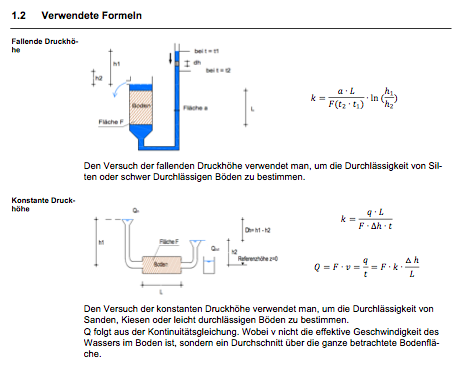
\includegraphics[width=\hsize]{kugel/Bild.png}
\caption{Kommentar zum Bild
\label{kugel:erstesbild}
}
\end{figure}

Im Bild \ref{kugel:erstesbild} sieht man BLAH:

Schon seit jeher fasziniert den Menschen die Fahrt zur See. Nicht grundlos ist die Seefahrt eine der wichtigsten und ältesten Tätigkeiten der Menschheit. Der innerliche Drang neue Weltmeere und unbekannte Gebiete zu entdecken, die Fahrt zur See zu erleichtern und erträglicher zu machen, trieben die Menschen an, die Schiffe dieser Welt immer weiter zu entwickeln.

Die Idee der Kugelform der Erde ist älter als man zu denken vermag. Bereits der Schüler des antiken griechischen Philosophen Platon - Aristoteles schrieb in seiner Schrift \textit{Über den Himmel} aus dem 4. Jahrhundert v. Chr. etliche Gründe welche für die Gestallt der Erde als Kugel sprechen:

-Sämtliche schweren Körper streben zum Mittelpunkt des Alls. Da sie dies von allen Seiten her gleichmäßig tun und die Erde im Mittelpunkt des Alls steht, muss sie eine kugelrunde Gestalt annehmen.
- Bei von der Küste wegfahrende Schiffen wird der Rumpf vor den Segeln der Sicht verborgen.
- In südlichen Ländern erscheinen südliche Sternbilder höher über dem Horizont.
- Der Erdschatten bei einer Mondfinsternis ist stets rund.

Jedoch war um 1492 - der Zeit der Entdeckung Amerikas durch Christoph Kolumbus, die Idee der Erde in Kugelform noch sehr umstritten. Er erkannte anhand den Theorien und Erkenntnissen der alten Griechen, vor allem Aristoteles, das die Erde eine Kugel sein muss. 
Doch mit seinem Vorschlag einen Seeweg über den Atlantik nach Indien zu finden und nicht wie üblich um Afrika zu segeln, stiess er beim beim portugiesischen König auf taube Ohren. Sein Plan Indien über eine Route nach Westen zu erreichen, widersprach dem gesunden Menschenverstand. Wäre die Erde wirklich eine Kugel und man befände sich auf der unteren Erdhalbkugel, würde man herunterfallen.
Doch auch der damals übliche Glaube an die Erde in Scheibenform brachte so einige Risiken mit sich. Was würde passieren, wenn die Flotte das Ende der Scheibe erreicht hatte? Würden sie über den Erdrand hinweggleiten und in den Abgrund stürzen?
Erst nach viel Überzeugungsarbeit durch Kolumbus, setzte er sich am Spanischen Hof durch und segelte über die Westliche Route über den Atlantik und entdeckte schlussendlich Amerika.

Der praktische und greifbare Beweis das die Erde eine Kugel ist, lieferte rund 30 Jahre später der Portugiese Fernando Magellan. Mit seiner Weltumsegelung und seiner Ankunft in den Philippinen, bewies er definitiv das die Erde eine Kugel ist.

Nun wollen wir uns die Frage stellen, wie die alten Seefahrer ohne GPS und jeglichen modernen Navigationssystemen auf hoher See wussten wo sie sich befinden und was haben die Sterne mit alldem zu tun?

Reisen Sie mit uns zurück in eine Zeit mit Sextant, Kompass und Sternkarten. In die Zeit der Seefahrer und Entdecker.


\section{Geometrie auf der Ebene und der Kugel}

Euklid von Alexandria beschrieb die Grundbegriffe der ebenen Geometrie mittels Punkt, Geraden, Ebene, Winkel und Dreieck. Diese Dreiecke lassen sich mithilfe der ebenen Trigonometrie beschreiben.

Dabei gelten die uns bekannten trigonometrischen Winkelfunktionen:

\textbf{Sinussatz}
$\frac{ a }{ sin(\alpha) } = \frac{ b }{sin(\beta)} = \frac{ c }{ sin(\gamma) } = \frac{abc}{2A} = 2r$

\textbf{Cosinussatz}
$c^{ 2 } = a^{ 2 } + b^{ 2 } - 2*a*b*cos(\gamma)
b^{ 2 } = a^{ 2 } + c^{ 2 } - 2*a*b*cos(\beta)
a^{ 2 } = b^{ 2 } + c^{ 2 } - 2*a*b*cos(\alpha)$

Um Dreiecke auf der Kugeloberfläche zu berechnen, benötigt man die sphärische Trigonometrie. Die oben beschriebenen Sätze lassen sich auf der Kugel nicht anwenden, sie werden aber als Grundlage zur Herleitung der Sätze für das Kugeldreieck benötigt.

Die nachfolgenden Seiten thematisieren die Geometrie auf der Kugeloberfläche und wie sie in der Navigation eingesetzt werden kann.


\section{Gross- und Kleinkreise}

Eine Kugeloberfläche lässt sich in zwei verschiedene Kreisarten einteilen -  Gross- und Kleinkreise. 
Wir betrachten als erstes die Grosskreise:

\begin{definition}
Ein Großkreis ist ein größtmöglicher Kreis auf einer Kugeloberfläche. Sein Mittelpunkt fällt immer mit dem Mittelpunkt der Kugel zusammen und ein Schnitt auf dem Großkreis teilt die Kugel in jedem Fall in zwei („gleich große“) Hälften.
\end{definition}

Es gibt unendlich viele Möglichkeiten, eine Kugel in zwei gleich grosse Stücke zu zerschneiden, 
daher gibt es auch unendlich viele Grosskreise. Wenn wir die Grosskreise auf einer Kugel mit diesen auf der Erde beschreiben, sprechen wir von den Längengraden aber auch der Äquator beschreibt einen Grosskreis.
Ein Elementarer Bestandteil bilden die Grosskreise in der sphärischen Trigonometrie. Mithilfe der Schnittpunkte verschiedener Grosskreise, lässt sich ein Sphärisches Dreieck bilden auf welchem sich die sphärische Trigonometrie anwenden lässt.

[GRAFIK GROSSKREISE]

\begin{definition}
Unter Kleinkreis versteht man jene Kreise auf einer Kugeloberfläche, deren Ebenen nicht den Kugelmittelpunkt enthalten.
\end{definition}

Die Kleinkreise eignen sich im Gegensatz zu den Grosskreisen \textit{nicht} für die sphärische Trigonometrie. 
Sie werden lediglich zur Bestimmung der Messgrössen, Winkelabstände oder des Höhenwinkels eines Gestirns verwendet. 

Wenn wir die Kleinkreise auf die Erdoberfläche projizieren betrachten wir die Breitengrade.

[GRAFIK KLEINKREISE]


\section{Sphärische Dreiecke / Kugeldreieck}

[GRAFIK EULERSCHE DREIECK; ZWEIECK; NICHT EULERSCHES DREIECK]

Der Begriff Sphärisches Dreieck oder Kugeldreieck ist ein sehr weitläufiger Begriff. 
Dabei können wir den Begriff in drei für uns wesentliche Dreiecke unterteilen:

$\cdot Kugelzweieck$
$\cdot Eulersche’Dreiecke / Nicht Eulersche’Dreiecke$
$\cdot Grenzfall$


\subsection{Kugelzweieck}

Zwei Grosskreise auf der Kugeloberfläche, zerlegen diese in vier gleiche Kugelzweiecke. 
Jedes dieser Dreieckseiten hat die Länge
$180^{\circ}$ oder $\pi$
Der Flächeninhalt wird dabei nur durch den Winkel $\alpha$ zwischen den beiden Grosskreisen bestimmt.
Dabei ist der Flächeninhalt der ganzen Kugel:

$A_{ Kugel } = 4 \pi r^{2}$

Um den Flächeninhalt des betrachteten Zweieckes zu bekommen, 
müssen wir das ganze noch mit dem Kugelsegment mit dem Winkel $\alpha$ multiplizieren.

$A_{ Zweieck } = 4 \pi r^{2} * \frac{ \alpha }{ 2 \pi }$


\subsection{Eulersche Dreiecke / Nicht Eulersche’Dreiecke}

%[SKIZZE DER DREI GROSSKREISE WELCHES EIN EULERSCHES DREIECK BILDEN! SKIZZE DER VERSCHIEDENEN DREIECKEN]

Legt man drei Grosskreise auf eine Kugeloberfläche, bilden sich dabei acht Dreiecke. 
Ein solches Dreieck heisst Eulersches’Dreieck\footnote{%
Leonard Euler (1707-1783), berühmter Schweizer Mathematiker und Physiker. 
Nicht Eulersche’Dreiecke erhält man, indem man das Äussere des Dreieckes ABC betrachtet.} 
Diese Dreiecke werden weder durch die Verlängerung ihrer Seiten durchschnitten, 
noch haben sie Dreiecksseiten welche grösser als $180^{\circ}$ sind.

In den nachstehenden Erklärungen und Herleitungen, sprechen wir ausschliesslich von Eulerschen’Dreiecken, da die umgeformten Winkelsätze der ebenen Trigonometrie nur auf diese Art von Kugeldreiecken angewendet werden kann.

[GRAFIK]


\begin{align*}
\text{Zweieck} A
&=
\overline{ABC} + \overline{A'BC} = 2\alpha r^{ 2 } = A_{ \alpha }\\
\text{Zweieck}B
&=
\overline{ABC} + \overline{AB'C} = 2\beta r^{ 2 } = A_{ \beta }\\
\text{Zweieck}C
&=
\overline{ABC} + \overline{ABC'} = 2\gamma r^{ 2 } = A_{ \gamma }
\end{align*}

\begin{align*}
A_{ \alpha } + A_{ \beta } + A_{ \gamma } &= \frac{ 4\pi r^{ 2 } }{ 2 } + 2A_{ \overline{ ABC }} \\
2\alpha r^{ 2 } + 2\beta r^{ 2 } + 2\gamma r^{ 2 } &= \frac{ 4\pi r^{ 2 } }{ 2 } + 2A_{ \overline{ ABC }} \parallel:2\\
\alpha r^{ 2 } + \beta*r^{ 2 } + \gamma*r^{ 2 } &= \pi*r^{ 2 } + A_{ \overline{ ABC }} \parallel-\pi r^{ 2 }\\
r^{ 2 }\left(\alpha + \beta + \gamma - \pi\right) &= A_{ \overline{ ABC }}
\end{align*}

$A_{ \overline{ ABC }}$ ist die Fläche des Dreieckes auf der Kugeloberfläche


In der ebenen Trigonometrie liegt die Winkelsumme eines Dreiecks bei
$180^{\circ}$

Anders aber in der sphärischen Trigonometrie. Obschon sie einige Gemeinsamkeiten zur ebenen Trigonometrie aufweist, kann man nicht alles übernehmen.
So auch nicht wie Winkelsumme in einem sphärischen Dreieck. Diese liegt bei:

$\pi / 180^{\circ} bis 3\pi / 540^{\circ}$

daraus lässt sich ableiten, das ein einzelner Winkel nicht grösser sein darf als

$\pi / 180^{\circ}$ 

sein kann. Ansonsten ist es ein sphärisches Zweieck.
Wichtig anzumerken ist, dass die Seiten immer in Radiant
beschrieben werden und nicht im Längenmass Meter oder Kilometer wie wir es uns gewohnt sind. 
Denn bei den Seiten handelte es sich um Kreisbögen, welche in Radiant angegeben werden.


\subsection{Grenzfall - Satz von Legendre}

\textit{Ein kleines sphärisches Dreieck kann näherungsweise 
wie ein ebenes Dreieck mit denselben Seiten berechnet 
werden, wenn alle Winkel des ebenen Dreiecks die um 
je ein Drittel des sphärischen Exzesses verminderten 
Winkel des sphärischen Dreiecks nimmt.}

- Paris, 1787, Adrien-Marie Legendre (1752-1833)


Diese Aussage zeigt den Zusammenhang zwischen der 
Trigonometrie in der Ebene sowie in auf der Kugel
auf. Im speziellen bei sehr kleinen sphärischen 
Dreiecken ist die Winkelsumme nur unwesentlich 
grösser als $180^{\circ}$. Des Weiteren kann gesagt werden,
dass der sphärische Exzess gleichmässig auf alle
Winkel aufgeteilt wird.
Wichtig anzumerken ist, dass der Satz von Legendre 
für grosse, aber endliche Radien $r$ gilt.

%[SKIZZE GROSSER RADIUS/KLEINES DREIECK, KLEINER RADIUS/KLEINES DREIECK KRÜMMUNG!!!!]
%

\section{Sphärischer Exzess}

$\epsilon = \alpha + \beta + \gamma - \pi$

In der Ebenen Trigonometrie ist der Exzess = 0

Herleitung des spährischen Exzesses

Um den spährischen Exzess herzuleiten sind 
folgende Überlegungen notwendig.
Es wird davon ausgegangen, dass in einer Kugel
3 spährische Zweiecke abgebildet sind. Diese schneiden
sich drei mal und bilden 3 Eulersche’Dreiecke.

[Grafik]

\begin{align*}
Zweieck A
&=
\overline{ABC} + \overline{A'BC} = 2*\alpha*r^{ 2 } = A_{ \alpha }\\
Zweieck B
&=
\overline{ABC} + \overline{AB'C} = 2*\beta*r^{ 2 } = A_{ \beta }\\
Zweieck C
&=
\overline{ABC} + \overline{ABC'} = 2*\gamma*r^{ 2 } = A_{ \gamma }
\end{align*}

\begin{align*}
A_{ \alpha } + A_{ \beta } + A_{ \gamma }
&=
\frac{ 4\pi*r^{ 2 } }{ 2 } + 2A_{ \overline{ ABC }} 
\\
2*\alpha*r^{ 2 } + 2*\beta*r^{ 2 } + 2*\gamma*r^{ 2 }
&=
\frac{ 4\pi*r^{ 2 } }{ 2 } + 2A_{ \overline{ ABC }} \parallel:2
\\
\alpha*r^{ 2 } + \beta*r^{ 2 } + \gamma*r^{ 2 }
&=
\pi*r^{ 2 } + A_{ \overline{ ABC }} \parallel-\pi*r^{ 2 }
\\
r^{ 2 }*\left(\alpha + \beta + \gamma - \pi\right)
&=
A_{ \overline{ ABC }}
\end{align*}
ist die Fläche des Dreieckes auf der Kugeloberfläche.







\section{The Board of Longitude - Das Längenproblem}





\section{XX}




\section{XY}




\printbibliography[heading=subbibliography]
\end{refsection}



